%%%%%%%%%%%%%%%%%%%%%%%%%%%%%%%%%%%%%%%%%
% Journal Article
% LaTeX Template
% Version 1.4 (15/5/16)
%
% This template has been downloaded from:
% http://www.LaTeXTemplates.com
%
% Original author:
% Frits Wenneker (http://www.howtotex.com) with extensive modifications by
% Vel (vel@LaTeXTemplates.com)
%
% License:
% CC BY-NC-SA 3.0 (http://creativecommons.org/licenses/by-nc-sa/3.0/)
%
%%%%%%%%%%%%%%%%%%%%%%%%%%%%%%%%%%%%%%%%%

%----------------------------------------------------------------------------------------

%	PACKAGES AND OTHER DOCUMENT CONFIGURATIONS
%----------------------------------------------------------------------------------------
\documentclass[twoside,twocolumn]{article}

\usepackage[sc]{mathpazo} % Use the Palatino font
\usepackage[T1]{fontenc} % Use 8-bit encoding that has 256 glyphs
%\linespread{1.05} % Line spacing - Palatino needs more space between lines
\usepackage{microtype} % Slightly tweak font spacing for aesthetics

\usepackage[english]{babel} % Language hyphenation and typographical rules

\usepackage[hmarginratio=1:1,top=32mm,columnsep=20pt]{geometry} % Document margins
\usepackage[hang, small,labelfont=bf,up]{caption} % Custom captions under/above floats in tables or figures
\usepackage{booktabs} % Horizontal rules in tables

\usepackage{lettrine} % The lettrine is the first enlarged letter at the beginning of the text

\usepackage{enumitem} % Customized lists
\setlist[itemize]{noitemsep} % Make itemize lists more compact

\usepackage{abstract} % Allows abstract customization
\renewcommand{\abstractnamefont}{\normalfont\bfseries} % Set the "Abstract" text to bold
\renewcommand{\abstracttextfont}{\normalfont\small\itshape} % Set the abstract itself to small italic text

\usepackage{titlesec} % Allows customization of titles
\renewcommand\thesection{\Roman{section}} % Roman numerals for the sections
\renewcommand\thesubsection{\roman{subsection}} % roman numerals for subsections
\titleformat{\section}[block]{\large\scshape\centering}{\thesection.}{1em}{} % Change the look of the section titles
\titleformat{\subsection}[block]{\large}{\thesubsection.}{1em}{} % Change the look of the section titles

\usepackage{fancyhdr} % Headers and footers
%\pagestyle{fancy} % All pages have headers and footers
%\fancyhead{} % Blank out the default header
%\fancyfoot{} % Blank out the default footer
%\fancyhead[C]{Running title $\bullet$ May 2016 $\bullet$ Vol. XXI, No. 1} % Custom header text
%\fancyfoot[RO,LE]{\thepage} % Custom footer text

\usepackage{titling} % Customizing the title section

\usepackage{hyperref} % For hyperlinks in the PDF

\usepackage{graphicx}
\usepackage[tbtags]{amsmath}

%----------------------------------------------------------------------------------------
%	TITLE SECTION
%----------------------------------------------------------------------------------------

\setlength{\droptitle}{-4\baselineskip} % Move the title up

\pretitle{\begin{center}\Huge\bfseries} % Article title formatting
\posttitle{\end{center}} % Article title closing formatting
\title{Analysis of Quality Factor of Damped Pendulums} % Article title
\author{%
\textsc{Tian Ye} \\%\thanks{A thank you or further information} \\[1ex] % Your name
\normalsize Henry Samueli School of Engineering and Applied Science, Univ. California Los Angeles \\ % Your institution
\and % Uncomment if 2 authors are required, duplicate these 4 lines if more
\textsc{Chris Ong} \\%\thanks{Corresponding author} \\[1ex] % Second author's name
\normalsize College of Letters and Science, Univ. California Los Angeles \\ % Second author's institution
%\normalsize \href{mailto:jane@smith.com}{jane@smith.com} % Second author's email address
}
\date{November 14, 2017} % Leave empty to omit a date
\renewcommand{\maketitlehookd}{%
\begin{abstract}
\noindent In Classical Physics, a physical pendulum is a rigid body that is free to rotate around a single pivot. When the pendulum is displaced from its equilibrium position, it undergoes harmonic oscillation, given that the angle of displacement is small. Both amplitude and frequency of oscillation remain constant in an ideal simple harmonic oscillator. When a second force that is proportional to the velocity is acting on the body, it is known as a damped oscillation. This first portion lab aims to analyze the underdamped, overdamped, and critically damped motion of the pendulum. The second portion aims to compute and analyze the quality factor of a driven oscillation using various methods. 
\end{abstract}
}

%----------------------------------------------------------------------------------------

\begin{document}

% Print the title
\maketitle

%----------------------------------------------------------------------------------------
%	ARTICLE CONTENTS
%----------------------------------------------------------------------------------------

\section{Introduction}

This report discusses the resonance frequencies of a damped and undamped pendulum. The objective is to use the resonance frequency of a system to solve for the quality factor, or \textit{Q}, of the system.

\footnotesize
\begin{align}
Q &= \frac{1}{2}\tau \omega_r \\
Q &\approx \frac{\omega_0}{\Delta \omega} 
\end{align}
\normalsize

\noindent Where $\tau$ is the damping time, $\omega_r$ is the damped resonance frequency, $\omega_0$ is the undamped resonance frequency, and $\Delta \omega$ is the full width of the resonance.$\textsuperscript{[1]}$ 
%------------------------------------------------

\section{Methods}

The first portion of the experiment involves swinging an anchor-shaped wedge, both with and without damping effects from a pair of magnets. By setting the starting position of the pendulum so that it is within a single blade length of itself, we are able to apply small angle theorem. The tests were used to find the natural frequency of oscillation, $f_0$, and the necessary spacing of the damping magnets to achieve critical damping, respectively.


\noindent We next solved for the driving frequency of the system by placing the damping magnets at a spacing that would completely damp the oscillation within 5 to 10 seconds and recorded the damping time. We then drove the oscillation via a wave driver at various frequencies, recording the Lissajous figures at each frequency until it took upon the appearance of a circle, which occurs at the driving frequency of the system.

\hfill


\noindent Using Equation 1, we then solve for $Q$ using the data gathered from the various tests. We then plotted the frequencies of oscillation to solve for $\Delta \omega$. When the various frequencies are plotted together, a curve is created that peaks at the resonance frequency. The width of the curve when it is at $\frac{1}{\sqrt{2}}$ of its maximum height is $\Delta \omega$. Using this, we can then approximate $Q$ using Equation 2.

%------------------------------------------------

\section{Analysis}

To solve for $f_0$, we plot the angular displacement versus time graph for underdamped, overdamped, and critically damped oscillations.

\begin{figure}[!htbp]
    \centering
    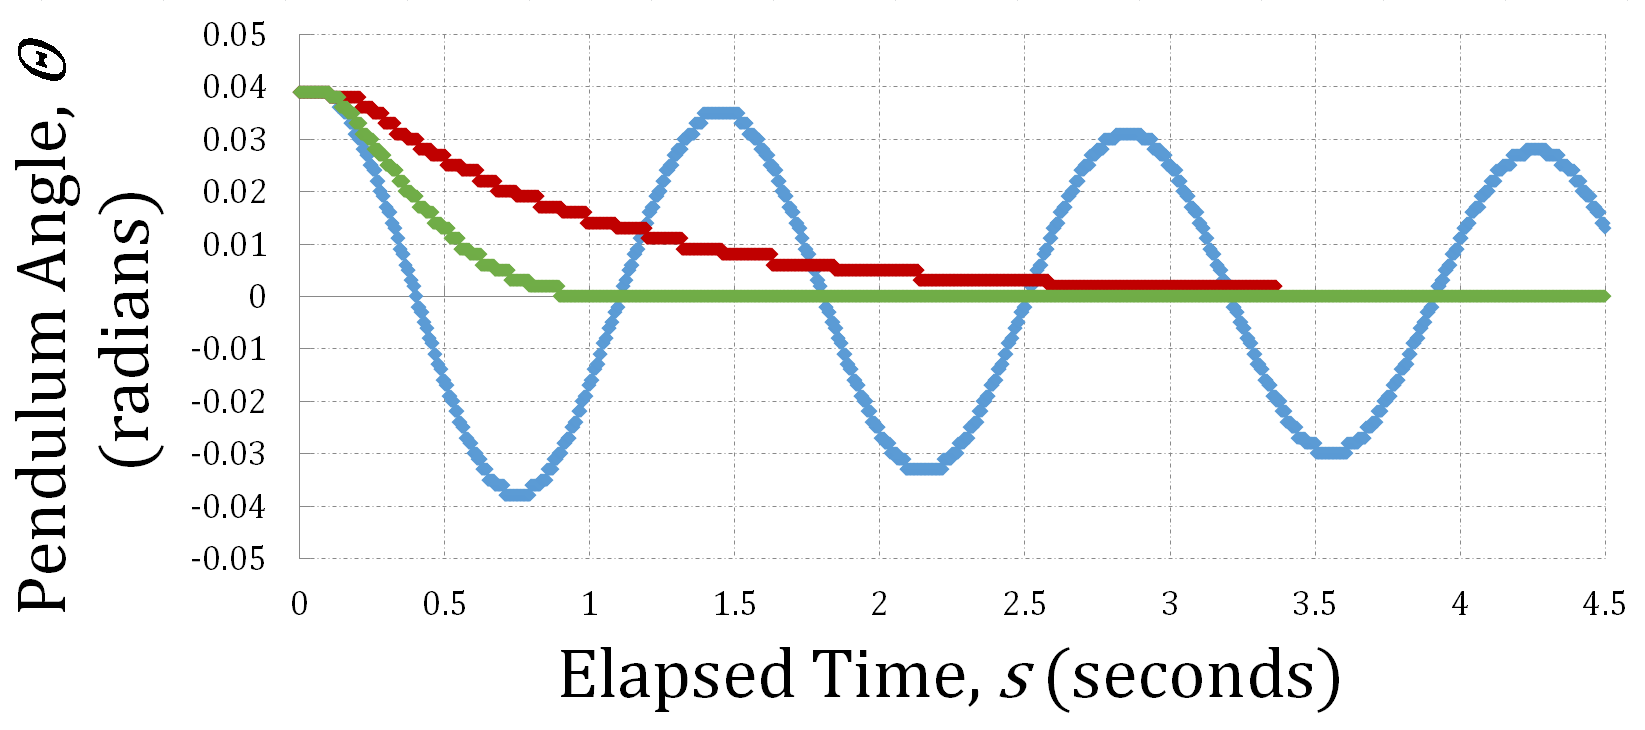
\includegraphics[width=2.9in]{ThreeFreq1.png}
    \caption{\textit{Solving for $f_0$ and critical damping spacing.} The blue curve represents the amplitude vs time graph of an underdamped oscillation, the red curve an overdamped oscillation, and the green curve a critically damped oscillation. The spacing between the magnets in the three tests are (50 $\pm$ 1) mm, (10 $\pm$ 1) mm, and (16 $\pm$ 1) mm, respectively.}
\end{figure}

\noindent Viewing the Figure 1, we can then solve for $f_0$ by finding the elapsed time interval between each maxima of the underdamped oscillation and dividing that value by the number of elapsed maxima minus 1. We then take the inverse of the period to solve for frequency. To normalize the data, we repeat this process for multiple ranges of extrema and solve for the uncertainty of our calculated frequency by using Equation ii.13 from the Lab Manual:

\footnotesize
\begin{equation}
\delta f = \frac{\sigma_f}{\sqrt{N}}
\end{equation}
\normalsize

\noindent Where $\sigma_f$ is the sample standard deviation and $N$ is the number of data points.$\textsuperscript{[1]}$ Using the methods described above, we find $f_0$ to be (0.713 $\pm$ 0.005) Hz. Therefore, by multiplying $f_0$ by $2\pi$, we find $\omega_0 = (4.48$ $\pm$ 0.03) Hz. 


\noindent We then find a spacing between the magnets so that an undriven oscillation completely dies out between 5 and 10 seconds before testing our driven oscillations. After several tests, we choose a separation between the magnets of (30 $\pm$ 1) mm. We then repeat the steps performed above to find the frequency of oscillation of the damped pendulum.

\begin{figure}[!htbp]
    \centering
    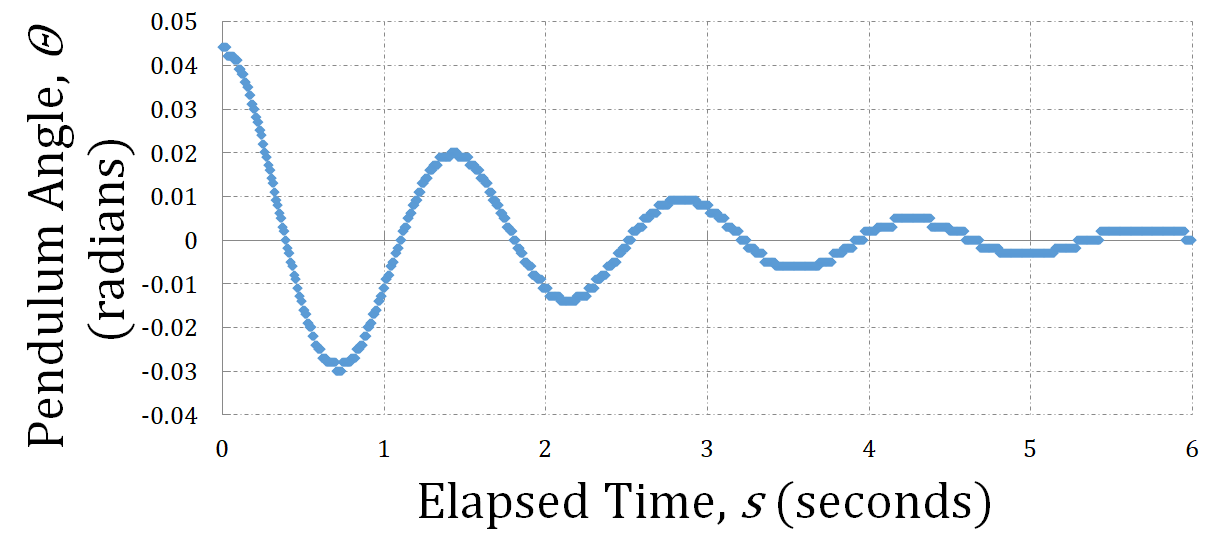
\includegraphics[width=2.9in]{DampedFreq.png}
    \caption{\textit{Solving for $f$ of damped oscillation.} The blue curve represents the amplitude vs time graph of the oscillation of the pendulum given the spacing between the damping magnets is (30 $\pm$ 1)mm.}
\end{figure}

\noindent From Figure 2 above, we calculate $f$ of the damped oscillation to be (0.718 $\pm$ 0.004) Hz. By isolating the amplitude of the successive maxima of the function, we are then able to calculate $r$, the ratio of successive maxima, to be 0.45 $\pm$ 0.01. Using this, we can then calculate the damping time, $\tau$, using the following equation:

\footnotesize
\begin{align}
\tau &= -\frac{T}{\text{ln}\Big [\frac{V(t+T)}{V(t)}\Big ]} \\
\tau &= -\frac{T}{\text{ln}[r]}
\end{align}
\normalsize

\noindent Where $r$ is the ratio of successive maxima. We find $\tau$ = (1.74 $\pm$ 0.01) s. Note: the high uncertainty value is due to the compounded uncertainty of the maxima of the function and the period of the function - both of which are due to the limitations of the recording devices and their precision.

\noindent Then, via the usage of Lissajous figures, we determine the resonance frequency of the system. 

\begin{figure}[!htbp]
    \centering
    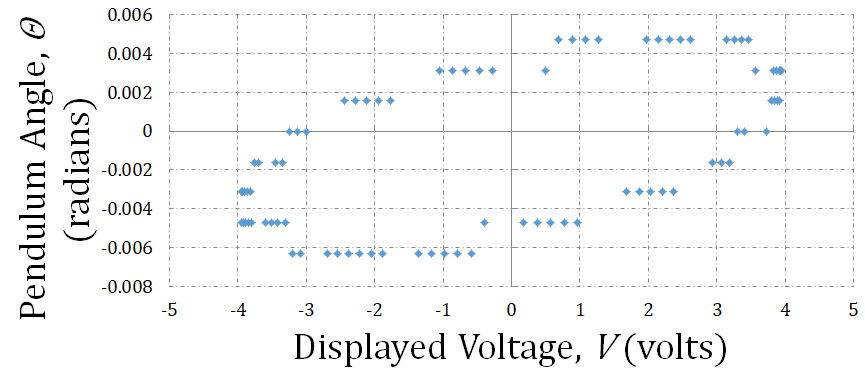
\includegraphics[width=2.9in]{FreqBelow.png}
    \caption{\textit{Solving for resonance frequency of driven oscillation.} The blue Lissajous figure corresponds to a driving frequency of 0.63 Hz.}
\end{figure}

\begin{figure}[!htbp]
    \centering
    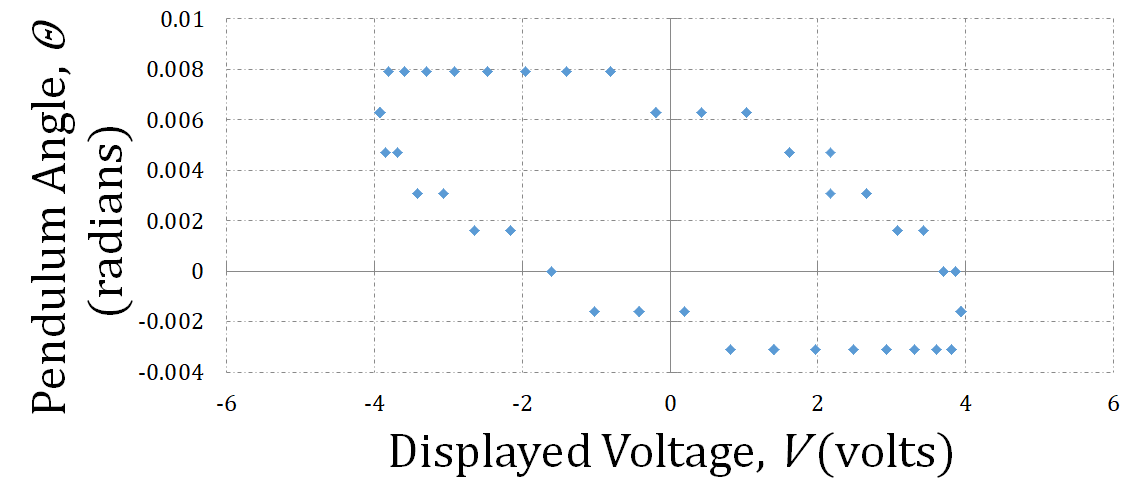
\includegraphics[width=2.9in]{FreqAbove.png}
    \caption{\textit{Solving for resonance frequency of driven oscillation.} The blue Lissajous figure corresponds to a driving frequency of 0.75 Hz.}
\end{figure}

\begin{figure}[!htbp]
    \centering
    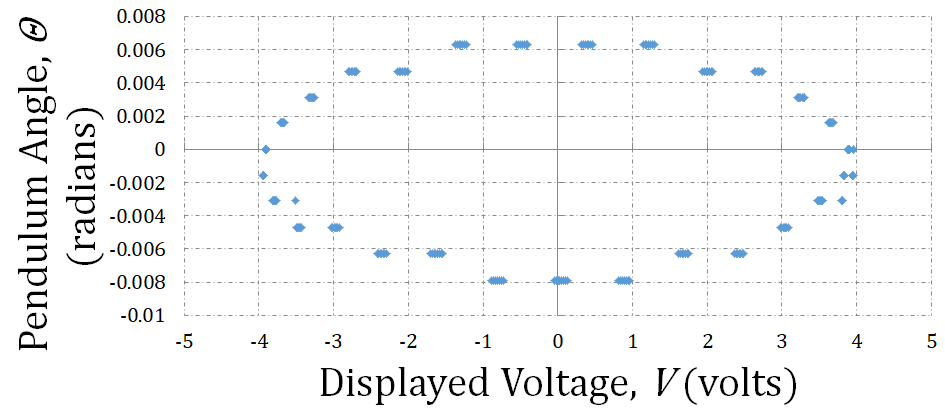
\includegraphics[width=2.9in]{FreqOn.png}
    \caption{\textit{Solving for resonance frequency of driven oscillation.} The blue Lissajous figure corresponds to a driving frequency of 0.69 Hz.}
\end{figure}

\noindent The ellipse of the Lissajous figure tilts depending on how far above or below resonance the current frequency is. Therefore, the Lissajous figure at resonance appears as a symmetrical ellipse with no slant, which in this case is the figure corresponding to the driving frequency of (0.690 $\pm$ 0.001) Hz. Given that, we then know that $\omega_r =$ (4.335 $\pm$ 0.006) Hz.

\noindent Referring back to Equation 1 and using the following equation, we find Q = (3.77 $\pm$ 0.01).

\begin{align}
\delta Q = \frac{1}{2}\sqrt{(\tau \delta \omega_r)^2 + (\omega_r \delta \tau)^2}
\end{align}

\begin{figure}[!htbp]
    \centering
    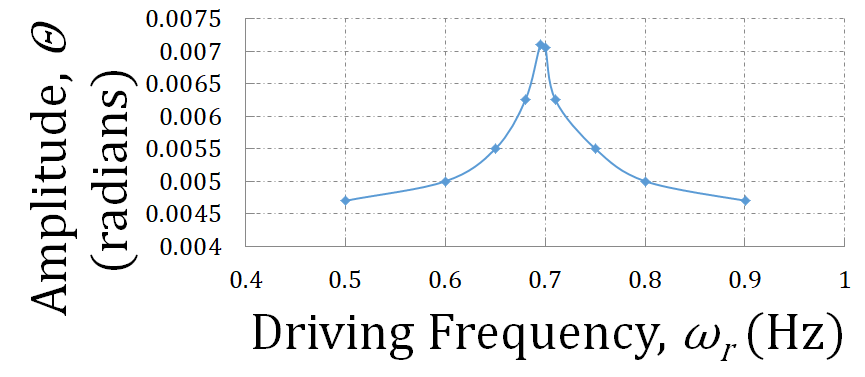
\includegraphics[width=2.9in]{Amplitude.png}
    \caption{\textit{Solving for $\Delta \omega$.} The curve is amplitude with respect to driving frequency.}
\end{figure}

\noindent We then use a second method to solve for the Q value via plotting the range of the amplitude frequencies.
\noindent Using Figure 6, we can now approximate $\Delta \omega$, the width of the graph when the curve is at $\frac{1}{\sqrt{2}}$ of its maximum amplitude. In this case, $\Delta \omega = (1.26$ $\pm$ 0.12) Hz, following the conversion from frequency to angular frequency.

\noindent Referring back to Equation 2 and using the following equation, we find Q = (3.45 $\pm$ 0.16).

\begin{align}
\delta Q = \frac{1}{2}\sqrt{\bigg (\frac{\omega_0}{\Delta \omega^2}\delta \Delta \omega)^2 + \bigg(\frac{1}{\Delta \omega} \delta \omega_0 \bigg)^2}
\end{align}

\noindent Using a third method to solve for Q, we adjust the driving frequency until the amplitude of the pendulum is approximately $\frac{1}{\sqrt{2}}$ of the maximum amplitude.

\begin{figure}[!htbp]
    \centering
    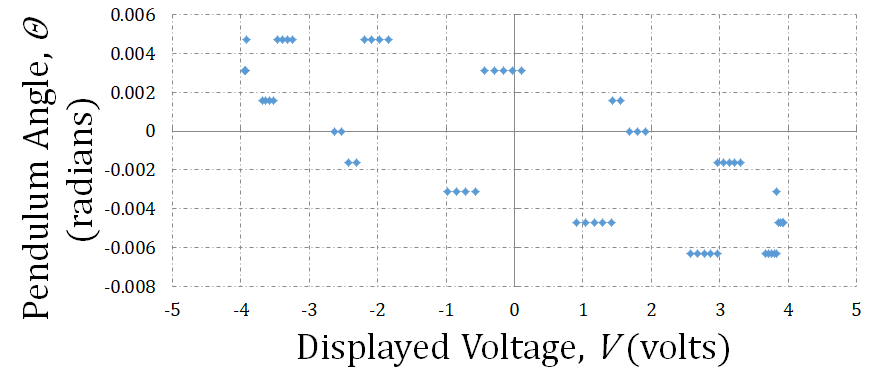
\includegraphics[width=2.9in]{ECAbove.png}
    \caption{\textit{Solving for $\Delta \omega$ of amplitude response curve.} The blue Lissajous figure corresponds to a driving frequency of 0.765 Hz.}
\end{figure}

\begin{figure}[!htbp]
    \centering
    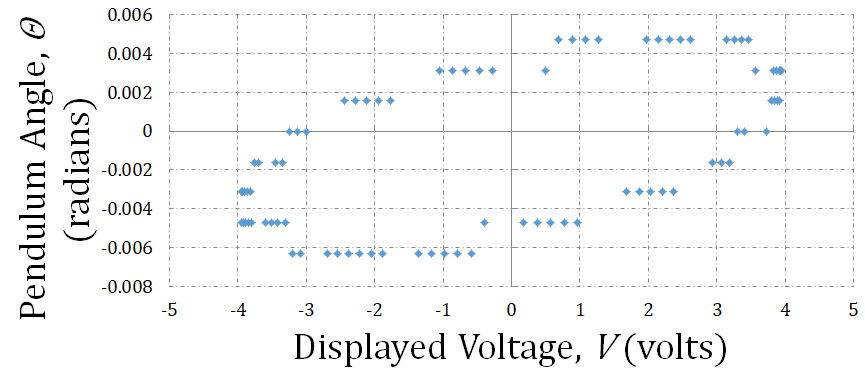
\includegraphics[width=2.9in]{FreqBelow.png}
    \caption{\textit{Solving for $\Delta \omega$ of amplitude response curve.} The blue Lissajous figure corresponds to a driving frequency of 0.625 Hz.}
\end{figure}

\noindent The figures are both elliptical and tilt in opposite directions. Furthermore, if the midpoint between the two frequencies are taken, we find that the resonance frequency found using this method is 0.695 Hz, which is similar to the value calculated earlier. Using this, we find $\Delta \omega$ to be 0.88 Hz. Using Equation 6.15 from the Lab Manual, we find a third Q value of (4.92 $\pm$ 0.3).

%------------------------------------------------

\section{Discussion}

\noindent When we compare the two Q values that were obtained from Equation 1 and Equation 2, we find that there is a nontrivial discrepancy between the values. The value derived from Equation 1 however is likely to be more accurate than the value derived from Equation 2, as the Q value derived from Equation 2 is heavily dependent on estimation of $\Delta \omega$. Due to that fact the uncertainty of $\Delta \omega$ has a large effect on the uncertainty of the Q value derived from Equation 2. When comparing the uncertainties as a percentage of the Q value for the Q values obtained from both Equation 1 and Equation 2, we find that the percentages are 0.2$\%$ and 4.6$\%$, respectively.

\hfill

\noindent While the Q value obtained from the third method is most different from the other two, it is more likely more accurate than the others, primarily due to the fact that it does not require guessing at the resonance frequency via visual analysis of Lissajous figures as is the limiting factor in the first method, and does not require guessing at a value of $\Delta \omega$ visually, as the second method requires. Furthermore, it is not constrained to only values of Q that are significantly greater than 1, as is in the case of Equation 2.

\hfill

\noindent Viewing the values of the quality factors themselves, we note that they are both relatively low. This implies that the oscillations are of a similar order magnitude and that they both quickly damped to 0, both of which are true for the case of this experiment.

\hfill

\noindent A primary source of systematic uncertainty in this experiment is the potential difference in recording times of the wave driver and rotation sensor for the Lissajous figures. The analysis on the current figures is operated under the assumption that both the data points for the voltage from the wave driver and the angle measured from the rotation sensor are being recorded at the same instance of time. However, if one is earlier than the other, it will in turn skew the tilt of the Lissajous figure and consequently skew the estimated resonance frequency of the pendulum.

\hfill

\noindent A second source of systematic uncertainty is friction between the pivot of the pendulum and the pendulum itself, which in turn creates its own damping force that is a function of the amplitude of oscillation. This would in turn indicate that as the pendulum approaches steady state, the force of damping from friction increases as well, which in turn skews the resonance frequency and consequently the Q value obtained from Equation 1.


%----------------------------------------------------------------------------------------
%	REFERENCE LIST
%----------------------------------------------------------------------------------------

\begin{thebibliography}{99} % Bibliography - this is intentionally simple in this template

\bibitem{1}
Campbell, W. C. \textit{et al}. Physics 4AL: Mechanics Lab Manual (ver. August 31, 2017).
(Univ. California Los Angeles, Los Angeles, California).

\end{thebibliography}

%----------------------------------------------------------------------------------------

\end{document}
